\documentclass[12pt,oneside]{uhthesis}
%\usepackage{biblatex}
\bibliography{Bibliography} % Entries are in the refs.bib file

\usepackage{subfigure}
\usepackage[ruled,lined,linesnumbered,titlenumbered,algochapter,spanish,onelanguage]{algorithm2e}
\usepackage{amsmath}
\usepackage{amssymb}
\usepackage{amsbsy}
\usepackage{caption,booktabs}
\captionsetup{ justification = centering }
%\usepackage{mathpazo}
\usepackage{float}
\setlength{\marginparwidth}{2cm}
\usepackage{todonotes}
\usepackage{listings}
\usepackage{xcolor}
\usepackage{multicol}
\usepackage{graphicx}
\usepackage{newclude}
\usepackage[utf8]{inputenc}
\floatstyle{plaintop}
\restylefloat{table}
%\addbibresource{Bibliography.bib}
% \setlength{\parskip}{\baselineskip}%
\renewcommand{\tablename}{Tabla}
\renewcommand{\listalgorithmcfname}{Índice de Algoritmos}
%\dontprintsemicolon
\SetAlgoNoEnd

\definecolor{codegreen}{rgb}{0,0.6,0}
\definecolor{codegray}{rgb}{0.5,0.5,0.5}
\definecolor{codepurple}{rgb}{0.58,0,0.82}
\definecolor{backcolour}{rgb}{0.95,0.95,0.92}

\lstdefinestyle{mystyle}{
    backgroundcolor=\color{backcolour},   
    commentstyle=\color{codegreen},
    keywordstyle=\color{purple},
    numberstyle=\tiny\color{codegray},
    stringstyle=\color{codepurple},
    basicstyle=\ttfamily\footnotesize,
    breakatwhitespace=false,         
    breaklines=true,                 
    captionpos=b,                    
    keepspaces=true,                 
    numbers=left,                    
    numbersep=5pt,                  
    showspaces=false,                
    showstringspaces=false,
    showtabs=false,                  
    tabsize=4
}

\lstset{style=mystyle}

\title{Generación automática de procesos de integración de datos. Inferencia de Joins}
\author{\\\vspace{0.25cm}Jes\'us Santos Capote}
\advisor{\\\vspace{0.25cm}Lic. Víctor Manuel Cardentey Fundora\\\vspace{0.2cm}Dra. C. Lucina García Hernández}
\degree{Licenciado en Ciencia de la Computación}
\faculty{Facultad de Matemática y Computación}
\date{Fecha\\\vspace{0.25cm}\href{https://github.com/username/repo}{https://github.com/JesusSantosCapote/autoETL.git}}
\logo{Graphics/uhlogo}
\makenomenclature

\renewcommand{\vec}[1]{\boldsymbol{#1}}
\newcommand{\diff}[1]{\ensuremath{\mathrm{d}#1}}
\newcommand{\me}[1]{\mathrm{e}^{#1}}
\newcommand{\pf}{\mathfrak{p}}
\newcommand{\qf}{\mathfrak{q}}
%\newcommand{\kf}{\mathfrak{k}}
\newcommand{\kt}{\mathtt{k}}
\newcommand{\mf}{\mathfrak{m}}
\newcommand{\hf}{\mathfrak{h}}
\newcommand{\fac}{\mathrm{fac}}
\newcommand{\maxx}[1]{\max\left\{ #1 \right\} }
\newcommand{\minn}[1]{\min\left\{ #1 \right\} }
\newcommand{\lldpcf}{1.25}
\newcommand{\nnorm}[1]{\left\lvert #1 \right\rvert }
\renewcommand{\lstlistingname}{Ejemplo de código}
\renewcommand{\lstlistlistingname}{Ejemplos de código}

\begin{document}

\frontmatter
\maketitle

\begin{dedication}
    Dedicatoria
\end{dedication}
\begin{acknowledgements}
A mis padres, por estar siempre presentes brindando su amor y apoyo, por ser luz 
en momentos de dudas, por ser su prioridad bajo cualquier circunstancia. Al resto de mi 
familia por su cariño y preocupaci\'on por mi bienestar. 

A mi hermana Massiel, por su cariño incondicional, por estar siempre presente, 
por ser mi ejemplo a seguir como cient\'ifico de la computaci\'on y como persona. 

A mis compañeros de carrera, Kenny Villalobos, Ernesto Alfonso, Abraham Gonzalez, Jorge A. Soler, Diamis Alfonso 
y Sheyla Leyva por todas las alegr\'ias y momentos difíciles compartidos; por su amistad incondicional y por 
impulsarme a ser un mejor profesional.

A mis amigos por soportar todos los "hoy no puedo ir", por su cariño y atenciones, por ser refugio del 
estrés durante toda esta etapa.

A los buenos profesores que me he encontrado en estos cuatro años y que contribuyeron al profesional que soy hoy. 
A MATCOM por ser una segunda casa.
\end{acknowledgements}
\begin{opinion}
    El uso de la información como un arma estratégica constituye una necesidad en el mundo actual. En realidad, no es 
    imprescindible la presencia de un almacén de datos en una solución de inteligencia de negocios dada la 
    heterogeneidad de los escenarios. Sin embargo, es preciso tomar en consideración la contribución de los 
    datos factuales para evaluar el progreso de una organización, así como el propósito que persigue el 
    proceso de población en cuanto a la integración de los datos con vistas a la ulterior exploración 
    multidimensional acertada. La construcción y el mantenimiento de un almacén de datos no resulta 
    una tarea sencilla, mucho menos la creación de una herramienta extensible y genérica.

    El trabajo de diploma desarrollado por el estudiante Jesús Santos Capote propone un Lenguaje de 
    Dominio Específico (DSL, por sus siglas en inglés) para la integración de datos estructurados en el 
    contexto del diseño de almacenes de datos basados en el Modelo Multidimensional. El DSL concebido 
    hace uso de bases de datos relacionales, bases de datos no relacionales orientadas a grafos, así 
    como algoritmos de grafos para generar el código del almacén de datos descrito por el desarrollador. 
    Al respecto, cabe destacar la complejidad de la inferencia de los joins requeridos para la obtención 
    del almacén de datos integrados desde las fuentes de datos en correspondencia con el escenario 
    analítico de interés. Entre las principales características de la solución se encuentra la 
    extensibilidad, al ser posible adaptar fácilmente la generación de código para distintos sistemas 
    gestores SQL. Este resultado será utilizado para continuar desarrollando la línea de integración de 
    datos dentro del Grupo de Sistemas de Información e Inteligencia de Negocios de la Universidad de 
    La Habana.

    Para validar el DSL propuesto, el estudiante utilizó dos casos de uso obtenidos de la literatura 
    especializada en el diseño multidimensional. Para ambos casos, partiendo de un esquema relacional, 
    se diseñó un esquema multidimensional que satisficiera los requerimientos del negocio, se especificaron 
    los diseños utilizando el DSL y se obtuvo un código funcional en PostgreSQL que permitía la creación 
    del almacén de datos, así como su población mediante la utilización de procesos ETL.

    Para poder afrontar el trabajo, el estudiante tuvo que revisar literatura científica relacionada con 
    la temática, así como soluciones existentes y bibliotecas de software que pueden ser apropiadas para 
    su utilización. Todo ello con independencia y sentido crítico, determinando las mejores aproximaciones 
    y también las dificultades que presentan. Además, ha tenido que asimilar varias tecnologías de 
    programación en un tiempo relativamente corto, demostrando tener dominio de su tema de investigación y 
    capacidad para resolver problemas complejos. Jesús ha mostrado gran entusiasmo y curiosidad científica, 
    mejorando continuamente su solución y planteándose nuevos retos que potencien el desarrollo de 
    investigaciones futuras, ambas cualidades de un excelente científico e investigador.

    Por las razones antes expuestas se propone que le sea otorgada al estudiante Jesús Santos Capote la 
    calificación de Excelente (5 puntos) y, de esta manera, pueda obtener el título de Licenciado en 
    Ciencia de la Computación.

    \vspace{1,0cm}

    Lic. Víctor Manuel Cardentey Fundora	\hspace{1,0cm}		Dra. C. Lucina García Hernández
\end{opinion}
\begin{resumen}
El Big Data ha generado una transformación significativa en la industria y la ciencia, facilitando el 
análisis de voluminosos y complejos conjuntos de datos que son fundamentales para respaldar la toma de 
decisiones. Los almacenes de datos emergen como infraestructuras clave en la consolidación de información 
crítica para este fin. No obstante, su construcción conlleva desafíos inherentes, principalmente en los 
procesos de integración de datos, que se caracterizan por su complejidad, extensión temporal y susceptibilidad 
a errores. En respuesta a estas dificultades, se han desarrollado sistemas orientados a la automatización de 
estos procesos, proporcionando herramientas que alivian la carga de los desarrolladores.

Esta tesis propone un marco de trabajo para la automatización de la integración de datos, poniendo 
especial atención en la inferencia de "joins", uno de los retos más críticos en este ámbito, a través de la 
implementación de un lenguaje de dominio específico y la aplicación de teoría de grafos. Se detallan los aspectos 
técnicos de un prototipo implementado y se realiza una evaluación experimental que demuestra la efectividad de la 
solución propuesta.
\end{resumen}

\begin{abstract}
The field of Big Data has brought about a significant transformation in both industry and science, enabling the 
analysis of large and complex datasets that are essential for decision-making. Data warehouses have emerged as 
key infrastructures for consolidating critical information. However, their construction presents inherent 
challenges, particularly in data integration processes, characterized by complexity, time extension, and 
susceptibility to errors. In response to these difficulties, systems have been developed to automate these 
processes, providing tools that alleviate the burden on developers.

This thesis proposes a framework for automating data integration, with special attention to the inference of "joins", 
one of the most critical challenges in this field, through the implementation of a specific domain language and the 
application of graph theory. The technical aspects of an implemented prototype are detailed, and an experimental 
evaluation is conducted to demonstrate the effectiveness of the proposed solution
\end{abstract}
\include{FrontMatter/Contents}

\mainmatter

\chapter*{Introducción}\label{chapter:introduction}
\addcontentsline{toc}{chapter}{Introducción}

Desde finales del siglo XX, el crecimiento acelerado de Internet, la adopci\'on generalizada de computadoras 
personales y el desarrollo de las redes sociales ha provocado que una gran variedad de datos se produzca a un ritmo 
sin precedentes y en grandes vol\'umenes. 
Este fen\'omeno, conocido como "Big Data" \cite{beyer2012importance}, ha impactado significativamente en diversas 
esferas de la actividad humana, facilitando el desarrollo de soluciones adaptables a las necesidades de diferentes 
campos de la ciencia y organizaciones industriales y de servicios.

Al procesar estas grandes cantidades de datos, se genera información actualizada y relevante que puede ser empleada 
para elaborar nuevas hipótesis o descubrir tendencias, patrones y correlaciones ocultas en los datos. Con la aparición del 
Big Data, las técnicas de procesamiento y metodologías asociadas al análisis de datos han evolucionado para adaptarse a esta 
nueva realidad, ofreciendo formas más eficientes de manejar y analizar grandes cantidades de información.

El an\'alisis de datos act\'ua como el proceso subyacente que energiza a otras tecnolog\'ias y procesos, nutri\'endolos
de los conocimientos derivados. Tal es el 
caso de la Inteligencia de Negocios (Business Intelligence, BI), la cual es un enfoque integrador orientado a tecnolog\'ias (technology-driven) 
para examinar los datos y proporcionar información accionable que ayude a los ejecutivos, gerentes y otros usuarios corporativos 
a tomar decisiones comerciales informadas. La BI abarca una amplia gama de herramientas, aplicaciones y metodologías 
que permiten a las organizaciones recopilar datos de sistemas internos y fuentes externas, prepararlos para análisis, 
desarrollar y ejecutar consultas sobre los datos y crear informes, paneles y visualizaciones de datos\cite{negash2004business}. 

Un elemento esencial de BI es el Procesamiento Analítico en Línea (Online Analytical Processing, OLAP), una tecnología que 
permite a los usuarios realizar análisis complejos en grandes cantidades de datos. OLAP posibilita la exploración de datos 
multidimensionales, proporcionando una forma de segmentar y resumir los datos desde diferentes perspectivas. Admite 
operaciones analíticas avanzadas como el desglose (drill-down), la consolidación (roll-up) y el pivote, que ayudan a los 
usuarios a obtener información valiosa de sus datos.

Detrás del Procesamiento Analítico en Línea (OLAP) se encuentran los Almacenes de Datos (Data Warehouse), que son 
estructuras que permiten realizar de manera eficiente las operaciones OLAP. Su proceso de creaci\'on implica la 
recopilación, 
organización, integración y almacenamiento de datos provenientes de diversas fuentes en un repositorio centralizado. Este 
repositorio funciona como una base de datos consolidada y estructurada que brinda soporte a consultas y análisis eficientes. 
Además, establece una base sólida para actividades de OLAP y otras funciones de BI, al 
asegurar la consistencia de los datos, así como la integración y el almacenamiento de datos históricos.

\section{Motivaci\'on}

En Cuba, durante los \'ultimos años, se ha promovido la introducción de nuevas tecnologías en los procesos 
productivos como parte de la diversificación y modernización de la economía. Como resultado, tanto instituciones 
estatales como privadas, así como organizaciones, empresas y centros, han visto la necesidad de desarrollar un Almac\'en 
de Datos para aprovechar eficientemente los datos generados por su actividad económica.

La creación y mantenimiento de un Almacén de Datos implica la ejecución de los procesos ETL (Extracción, Transformación y 
Carga) para abastecerlo de datos. Estos procesos son fundamentales para garantizar la integridad y calidad de los datos 
almacenados. Sin embargo, la implementación manual de estos procesos puede presentar diversos desafíos
\cite{nwokeji2021systematic, dhaouadi2022data, kimball2004data}.

En primer lugar, la implementación manual de los procesos ETL puede resultar compleja debido a la necesidad 
de manejar múltiples fuentes de datos, transformarlos de acuerdo con las necesidades del almacén y cargarlos de manera 
eficiente. Para esto, se requiere un conocimiento profundo de las fuentes de datos y de las técnicas de 
transformación, captura y extracción.

La implementación manual de los procesos ETL es propensa a errores humanos. La manipulación de grandes 
volúmenes de datos aumenta el riesgo de errores, como omisiones, duplicaciones o inconsistencias en los datos cargados, lo 
cual compromete la calidad del almac\'en de datos. Asimismo, es bien sabido que la implementación de procesos ETL puede consumir una 
considerable cantidad de tiempo y recursos.

Existen herramientas que abordan estas limitaciones al ofrecer posibilidades para la automatización de procesos ETL. 
Sin embargo, en su mayoría, estas herramientas son servicios alojados en la nube de sus propietarios, lo cual 
dificulta su acceso y aprovechamiento por parte de las pequeñas y medianas empresas cubanas. Esto se debe a la 
existencia de bases de datos on premise en las empresas y a limitaciones financieras, entre otras, lo cual 
obstaculiza el tratamiento de los datos en la nube.

Frente a los desafíos inherentes de la programaci\'on manual de los procesos ETL, a la condiciones actuales
de la isla y al creciente auge de la automatización de procesos en el ámbito de la computación, resulta 
provechoso contemplar la creación de una herramienta para la generación automática de procesos ETL, que satisfaga 
las necesidades del empresariado nacional.

\section{Antecedentes}

En la facultad de Matemática y Computación de la Universidad de La Habana, la labor de investigación e innovación de 
los profesores del colectivo de Sistemas de Información se ha caracterizado no solo por su interrelación estrecha 
con el almacenamiento, el análisis y la obtención de información con vista a la toma de decisiones en diversos 
escenarios de aplicación, sino también por la creación de herramientas genéricas que contribuyan a agilizar los 
procesos de implementación y población de los repositorios de datos asociados a las soluciones analíticas de 
inteligencia de negocio. Al respecto, se encuentran los trabajos "Población genérica
de un Data Warehouse Empresarial"\cite{mijailmaster} y "Herramienta genérica para la población del 
Warehouse Informacional"\cite{lismaster}.

En el primero se propone un procedimiento para el diseño de procesos ETCL
(Extracci\'on, Transformaci\'on, Depuraci\'on y Carga) compuesto por acciones, tareas y subprocesos. 
Las acciones engloban todas las posibles transformaciones que se pueden 
aplicar a los datos, así como los diversos tipos de extracción y carga. Por otro lado, las tareas constituyen un 
conjunto de acciones, mientras que los subprocesos se componen de un conjunto de tareas. De esta forma, un proceso 
ETCL puede ser modelado como un conjunto de subprocesos.

Además, brinda la implementación de una herramienta genérica para la población del Data Warehouse Empresarial, basada en el 
diseño ETCL propuesto. La herramienta diseñada hace uso de la arquitectura pluggins\cite{noauthor_plug-architectures_nodate}, 
de modo que en su n\'ucleo se encuentra 
un agente ETCL encargado de ejecutar los subprocesos cuyas extensiones son los disitintos tipos de acciones.

En el segundo se propone una formalización matemático computacional para el modelo de datos multidimensional. Asimismo,
brinda la implementación de un ambiente de creación para el Warehouse Informacional que permite crear y administrar 
estructuras multidimensionales y gestionar los metadatos. En el ambiente se modela cada uno de los componentes del modelo 
dimensional como interfaces, que describen las funcionalidades y caracter\'isticas usuales, dejando el c\'omo a las 
implementaciones 
espec\'ificas para cada plataforma. Utiliza el patr\'on proxy o representante para implementar 
las interfaces que sirven de intermediarios entre el ambiente y la tecnología que alojar\'a el Data Warehouse.

La presente investigaci\'on est\'a enmarcada en la tem\'atica de los Almacenes de Datos, inspir\'andose en los trabajos 
referidos, teniendo en cuenta el estudio detallado de las características y  las etapas esenciales del proceso de 
población en su conjunto, así como los modelos de solución consecuentes con el estado del arte de la época.


\section{Problem\'atica}

La generaci\'on autom\'atica de procesos ETL(Extracción, Transformación y Carga) es una tem\'atica amplia que a d\'ia de hoy no cuenta con una soluci\'on 
universalmente aceptada. Al realizar un acercamiento a las herramientas de generación automática de ETL más relevantes, se puede
identificar un denominador común: la utilización de modelos conceptuales para la definición de los
escenarios ETL.

En este proyecto, se propone la automatización de los procesos ETL para alimentar un entorno analítico, siguiendo 
las mejores prácticas de la industria. Esto se llevará a cabo mediante la creación de un Lenguaje de Dominio 
Específico (Domain Specific Language, DSL), que permite describir el modelo conceptual multidimensional subyacente, 
y un marco de trabajo asociado, que actuará como enlace entre las fuentes de datos relaconales y el almacén de datos 
analíticos resultante. El propósito es generar el código ETL requerido para el 
proceso de población de manera eficiente.

Una tabla de un Almacén de Datos puede contener atributos de m\'ultiples tablas de las fuentes de datos y 
atributos como resultado de agregaciones o de la aplicaci\'on de otras funciones. Por tanto, la generaci\'on autom\'atica 
del proceso ETL encargado de poblar dicha tabla, pasa por la inferencia de los Joins necesarios para obtener los atributos 
que la componen. Luego, uno de los problemas primarios a resolver en 
el marco de la generaci\'on autom\'atica de procesos ETL es la inferencia de Joins, el cual en s\'i mismo es uno de 
los retos m\'as significativos de la disciplina y que ocup\'o la mayor\'ia del tiempo de investigación e implementación 
del presente trabajo. En la bibliografía consultada sobre inferencia de Join u otros recursos matemático-computacionales 
que pueden ser adaptados al efecto, existen propuestas interesantes que utilizan la teor\'ia de grafos para abordar 
el problema. 

El problema científico que motiva la realización de esta investigación es disponer de una herramienta que 
favorezca la población de los almacenes de datos a partir de la generación automática del proceso ETL sin 
acceder a la nube. Finalmente, la presente investigación intenta dar respuesta a la siguiente interrogante: 
¿será factible generar 
automáticamente la(s) consulta(s) asociada(s) a la ETL de interés con vistas a poblar el repositorio de datos 
correspondiente, apoy\'andose en un lenguaje de dominio espec\'ifico y la teor\'ia de grafos?

\section{Objetivos}

\subsection{Objetivo general}

Concebir y diseñar un lenguaje de dominio específico para la definici\'on de escenarios analíticos, as\'i como un marco 
de trabajo que permita realizar la integración de datos, haciendo énfasis en la inferencia de joins, 
con vistas a poblar automáticamente el almacén de datos.

\subsection{Objetivos Espec\'ificos}

\begin{enumerate}
    \item Profundizar e el marco te\'orico conceptual respecto a la integración de datos en las soluciones de 
        inteligencia de negocios.  
    \item Estudiar y comparar las principales herramientas que permiten la automatización de procesos ETL en la actualidad.
    \item Concebir y diseñar un lenguaje de dominio específico para la definici\'on de escenarios analíticos en 
        correspondencia con el modelo multidimensional de datos.
    \item Implementar un software que permita inferir y ejecutar los joins necesarios para la población del escenario 
        previamente definido.
    \item Evaluar cualitativa y experimentalmente la validez de la solución implementada, partiendo de los resultados 
        obtenidos.
\end{enumerate}

\section{Propuesta de soluci\'on}

Se propone utilizar un Lenguaje de Dominio Específico (DSL) como método para vincular los modelos relacionales y analítico
que intervienen en un proceso ETL. El DSL cuenta con estructuras gramaticales que permiten definir qu\'e atributos 
contienen las dimensiones y los hechos del escenario analítico y de qu\'e tablas obtenerlos desde las fuentes de datos.

El proceso de generación del c\'odigo ETL comienza convirtiendo la fuente de datos en un grafo, donde las tablas 
se representan como nodos y las relaciones entre las tablas se representan como aristas. Este grafo, junto con las 
definiciones realizadas mediante el DSL, se utilizan como entrada para un algoritmo que infiere los joins necesarios.

Una vez calculados los joins, se seleccionan los más adecuados y se generará el 
código SQL correspondiente para la población del escenario analítico especificado.

Finalmente, el sistema propuesto se encargará de ejecutar de manera planificada los códigos generados con el propósito de 
mantener actualizado el almacén de datos. 

\section{Estructura del documento}

El resto del documento se ha estructurado en cuatro capítulos que abordan las distintas fases por las que transitó la 
presente investigación. En el cap\'itulo 1 se realiza un acercamiento al marco te\'orico conceptual de los Sistemas de 
Inteligencia de Negocios (BIS). En el cap\'itulo 2 se lleva a cabo un estudio de la actualidad de la generaci\'on autom\'atica 
de procesos ETL, exponiendo las especificidades de las principales herramientas del mercado que tratan de solventar esta 
problem\'atica. El cap\'itulo 3 constituye el núcleo de la concepción general de la solución propuesta, así como el 
diseño de la primera aproximación del lenguaje de dominio específico y del método para la inferencia de joins 
aplicando la teoría de grafos. En el capítulo 4 se 
detallan los aspectos técnicos de la implementación de un prototipo del sistema y se realiza un análisis de la validez de 
la solución implementada mediante el desarrollo de experimentos. A modo de descenlace, se presentan las conclusiones,
que recogen los resultados obtenidos de acuerdo al cumplimiento de los objetivos propuestos, así como las recomendaciones, 
donde se propone un conjunto de temáticas como parte de la continuación del presente trabajo. Por último, se enumeran
las referencias bibliográficas que sustentan la base científica y metodológica de la solución propuesta.

% Business Intelligence section
\chapter{Marco Te\'orico Conceptual}\label{chapter:teoricframe}

En este capítulo se realiza un acercamiento a los Sistemas de Inteligencia de Negocios (BIS) y, en particular, 
a los procesos de integración de datos, los cuales son fundamentales como escenario de actuación de la presente 
investigación.

\chapter{Generaci\'on Autom\'atica de Procesos ETL}\label{chapter:auto-etl}

El ETL automático es un proceso que 
aprovecha la tecnología y las técnicas de automatización para agilizar y simplificar los procesos ETL. Tiene el objetivo 
de reducir el esfuerzo manual y el tiempo requerido por las formas tradicionales de ejecutar tareas de integración, 
as\'i como mejorar la eficiencia, precisión y escalabilidad de estos procesos.

Mediante el uso de algoritmos inteligentes, aprendizaje de m\'aquina y herramientas de automatización, las soluciones de 
ETL automático pueden manejar complejas transformaciones de datos, tareas de limpieza, enriquecimiento 
y validación de datos. Usualmente, estas soluciones proporcionan interfaces gráficas que permiten a los 
usuarios diseñar y configurar visualmente los flujos de trabajo de ETL, definiendo la secuencia de operaciones y 
transformaciones de datos a realizar.

Al automatizar el proceso, las 
organizaciones pueden reducir el tiempo y el esfuerzo requeridos para realizar tareas de integración de 
datos y enfocarse en las tareas de an\'alisis, lo que posibilita un procesamiento de datos más rápido, acceso más rápido 
a información y una toma de decisiones mejorada.

La escalabilidad es otra ventaja de la ETL automático. A medida que los volúmenes de datos aumentan, los procesos manuales 
tradicionales de ETL pueden tener dificultades para mantenerse al día con las demandas crecientes. Las soluciones de ETL 
automática, con la potencia del procesamiento en la nube, pueden manejar conjuntos de datos grandes de manera eficiente, 
lo que permite a las organizaciones ampliar sus capacidades de integración de datos sin comprometer el rendimiento.

En el presente cap\'itulo se examinan los componentes clave de una solución de ETL automático en la sección 
\ref{section:PrincipalComp}. Además, se lleva a cabo un análisis de algunas de las herramientas principales en el 
mercado de ETL automático en la sección \ref{section:actual_tools}. Por último, se realiza una comparación entre las 
herramientas analizadas, teniendo en cuenta sus características más relevantes, en la sección 
\ref{section:ToolsComparison}. 


\chapter{Concepción y Diseño}\label{chapter:proposal}

A partir de las ideas adquiridas con el estudio de las herramientas expuestas en el cap\'itulo \ref{chapter:auto-etl}, 
en el presente capítulo se aborda el diseño de un lenguaje de dominio específico para la definición de 
escenarios analíticos. Asimismo, se expone la concepción general del marco de trabajo \textbf{AutoETL} para la 
integración de datos de forma automática partiendo de un modelo analítico definido mediante el DSL, cuya estructura 
f\'isica almacenar\'a los datos integrados. Los escenarios analíticos que se definen son esquemas estrellas, que como 
se expuso en el cap\'itulo \ref{chapter:teoricframe} especifican las dimensiones y las tablas de hechos 
que conforman un almacén de datos. 

Las dimensiones, generalmente, están formadas por atributos de distintas tablas de
las fuentes de datos, por ejemplo, una dimension que expresa la ubicación geográfica
se forma mediante el join de las tablas municipio, provincia y país. En las bases de
datos relacionales con un diseño correcto, es usual encontrarse estos tres conjuntos de
entidades separados en tablas normalizadas, enlazadas mediante llaves foráneas, con
el objetivo de evitar duplicación de datos y anomalías durante la inserción, modificación
y eliminación. Por tanto, el proceso de selección de datos para la población de la
dimensión ubicación geográfica pasa por la ejecuci\'on de joins sobre las tablas municipio, provincia y país,
para poder extraer los datos desde una única tabla, es decir, denormalizar la red  
de tablas municipio, provincia y país que fue formada durante el proceso de normalización. 

En las tabla de hechos sucede algo similar, puede que los valores de un hecho se
encuentren en una sola tabla o que en su calculo intervengan atributos de múltiples
tablas de la fuente, en ese caso es necesario interrelacionar explícitamente todas las tablas que intervengan
en el cálculo del hecho en cuestión mediante joins.

Luego una parte fundamental del proceso de integración de datos para la población de un escenario analítico es
la implementación de estos joins. Precisamente, la inferencia de joins por parte del marco trabajo concebido es el centro de atención de la presente 
investigaci\'on. La inferencia de joins implica la identificaci\'on mediante algoritmos y el uso de estructuras de datos de 
las tablas que intervienen en una consulta y las condiciones de join entre dichas tablas.
AutoETL realiza el proceso de inferencia de joins durante la generaci\'on 
del c\'odigo SQL asociado a las consultas que poblar\'an el escenario analítico, apoy\'andose de la definición del mismo
mediante el lenguaje de dominio específico.


\chapter{Implementación y Experimentos}\label{chapter:implementation}

Después de concebir y diseñar una solución computacional, es necesario llevar a cabo una implementación 
práctica para evaluar su validez. En este capítulo, se exponen las consideraciones fundamentales y 
las tecnologías empleadas en el desarrollo de un prototipo de la solución propuesta. Asimismo, se analiza 
la viabilidad del prototipo a través de la discusión de los resultados obtenidos en una serie de experimentos.



\backmatter
\begin{conclusions}
    El objetivo fundamental de este trabajo fue realizar una primera aproximaci\'on a la generaci\'on 
    autom\'atica de procesos ETL mediante el enfrentamiento del problema de la inferencia de joins. 

    A partir del estudio del estado de arte sobre la inferencia de joins y la automatizaci\'on de procesos 
    ETL se diseña un lenguaje de dominio espec\'ifico para la definici\'on de escenarios anal\'iticos que 
    vincula el modelo relacional y el modelo dimensional, el cual constituye el principal aporte de la 
    presente investigaci\'on. Adem\'as, se desarrolló un prototipo funcional de un marco de trabajo extensible 
    e independiente de los sistemas de gestión de bases de datos. Este marco, partiendo de la definición de un 
    escenario analítico mediante el lenguaje de dominio específico concebido, es capaz de generar consultas para la 
    extracción 
    de datos y la creación de tablas, infiriendo adecuadamente una conjunto joins necesarios para estas consultas, 
    con el 
    objetivo de poblar automáticamente el escenario definido. Sin embargo, debido a limitaciones de tiempo, no se 
    logró concretar una implementación para la generación de pipelines que utilicen las consultas generadas, las 
    ejecuten en un orden lógico e inserten los datos extra\'idos en el sistema destino
    para lograr la población efectiva de los escenarios analíticos definidos.

    Se ejecutaron experimentos que permitieron establecer la validez de la propuesta realizada y evidenciaron el 
    correcto funcionamiento del prototipo implementado.
\end{conclusions}

\begin{recomendations}
A partir de los desafíos computacionales encontrados, así como de los resultados
obtenidos por el sistema desarrollado, se identifican nuevas líneas de investigación que
permitan mejorar la efectividad del marco de trabajo propuesto:

\begin{itemize}
    \item Implementaci\'on de un generador de pipelines, gen\'erico e independientes de los sistemas 
        de gestión de bases de datos, para la poblaci\'on automática de los escenarios analíticos definidos en los 
        que adem\'as se les pueda configurar el tipo de extracción de datos y de carga a utilizar.
        
    \item El prototipo implementado necesita la intervención del usuario para seleccionar los joins
        de las consultas de selecci\'on. Se propone la implementaci\'on de un sistema que permita 
        analizar la semántica de los joins computados y seleccione de forma autom\'atica el join 
        m\'as conveniente para la consulta que se ha de generar.

    \item Enriquecimiento del lenguaje de dominio espec\'ifico concebido para abarcar otros aspectos 
        de la definición de modelos dimensionales tales como la granularidad y la aditividad. 
        
    \item Enriquecimiento del lenguaje de dominio espec\'ifico y del marco de trabajo diseñado 
        para lograr la automatizaci\'on de otros procesos de la integraci\'on de datos, además de la inferencia 
        de joins.
\end{itemize}

\end{recomendations}

\begin{annexes}
    \begin{figure}
        \centering
        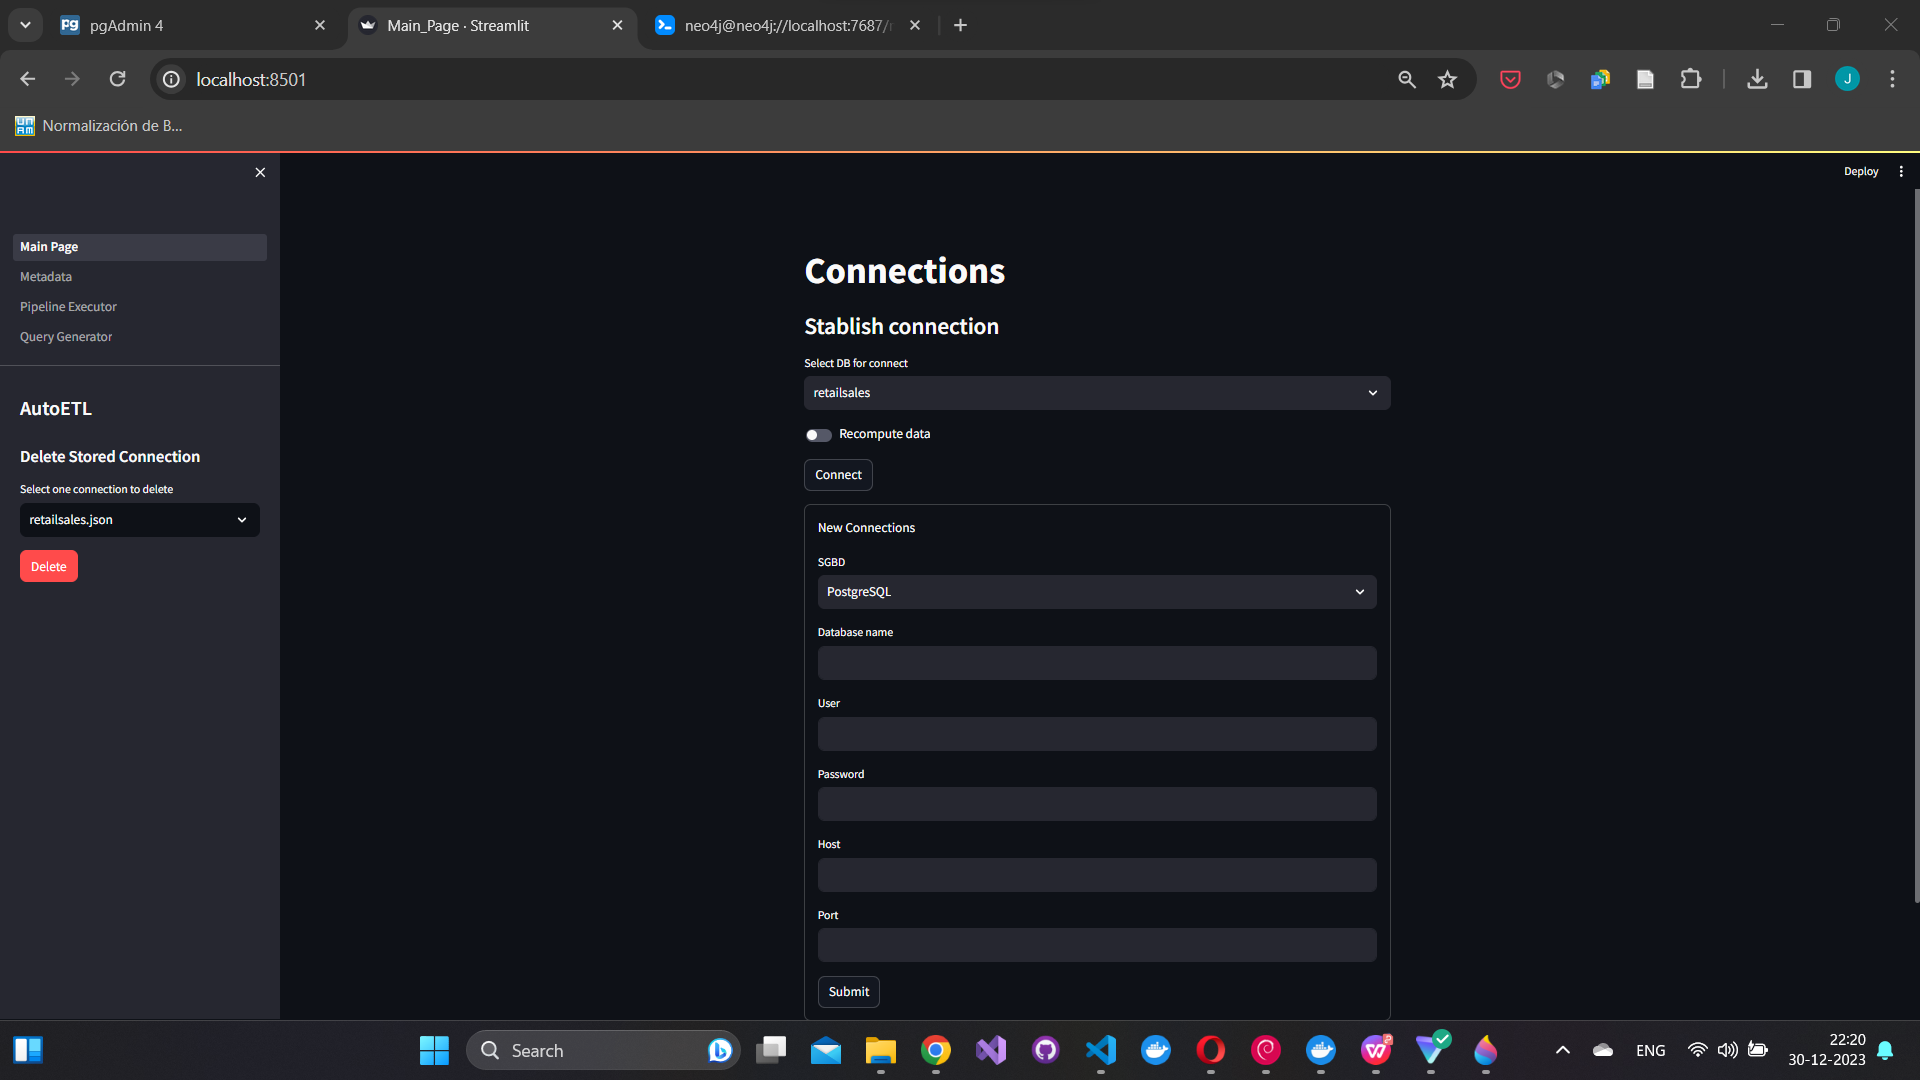
\includegraphics[scale=0.4]{Graphics/mainpage.png}
        \caption{Im\'agen de la p\'agina Main Page.}
        \label{fig:mainpage}
      \end{figure}

    \begin{figure}
        \centering
        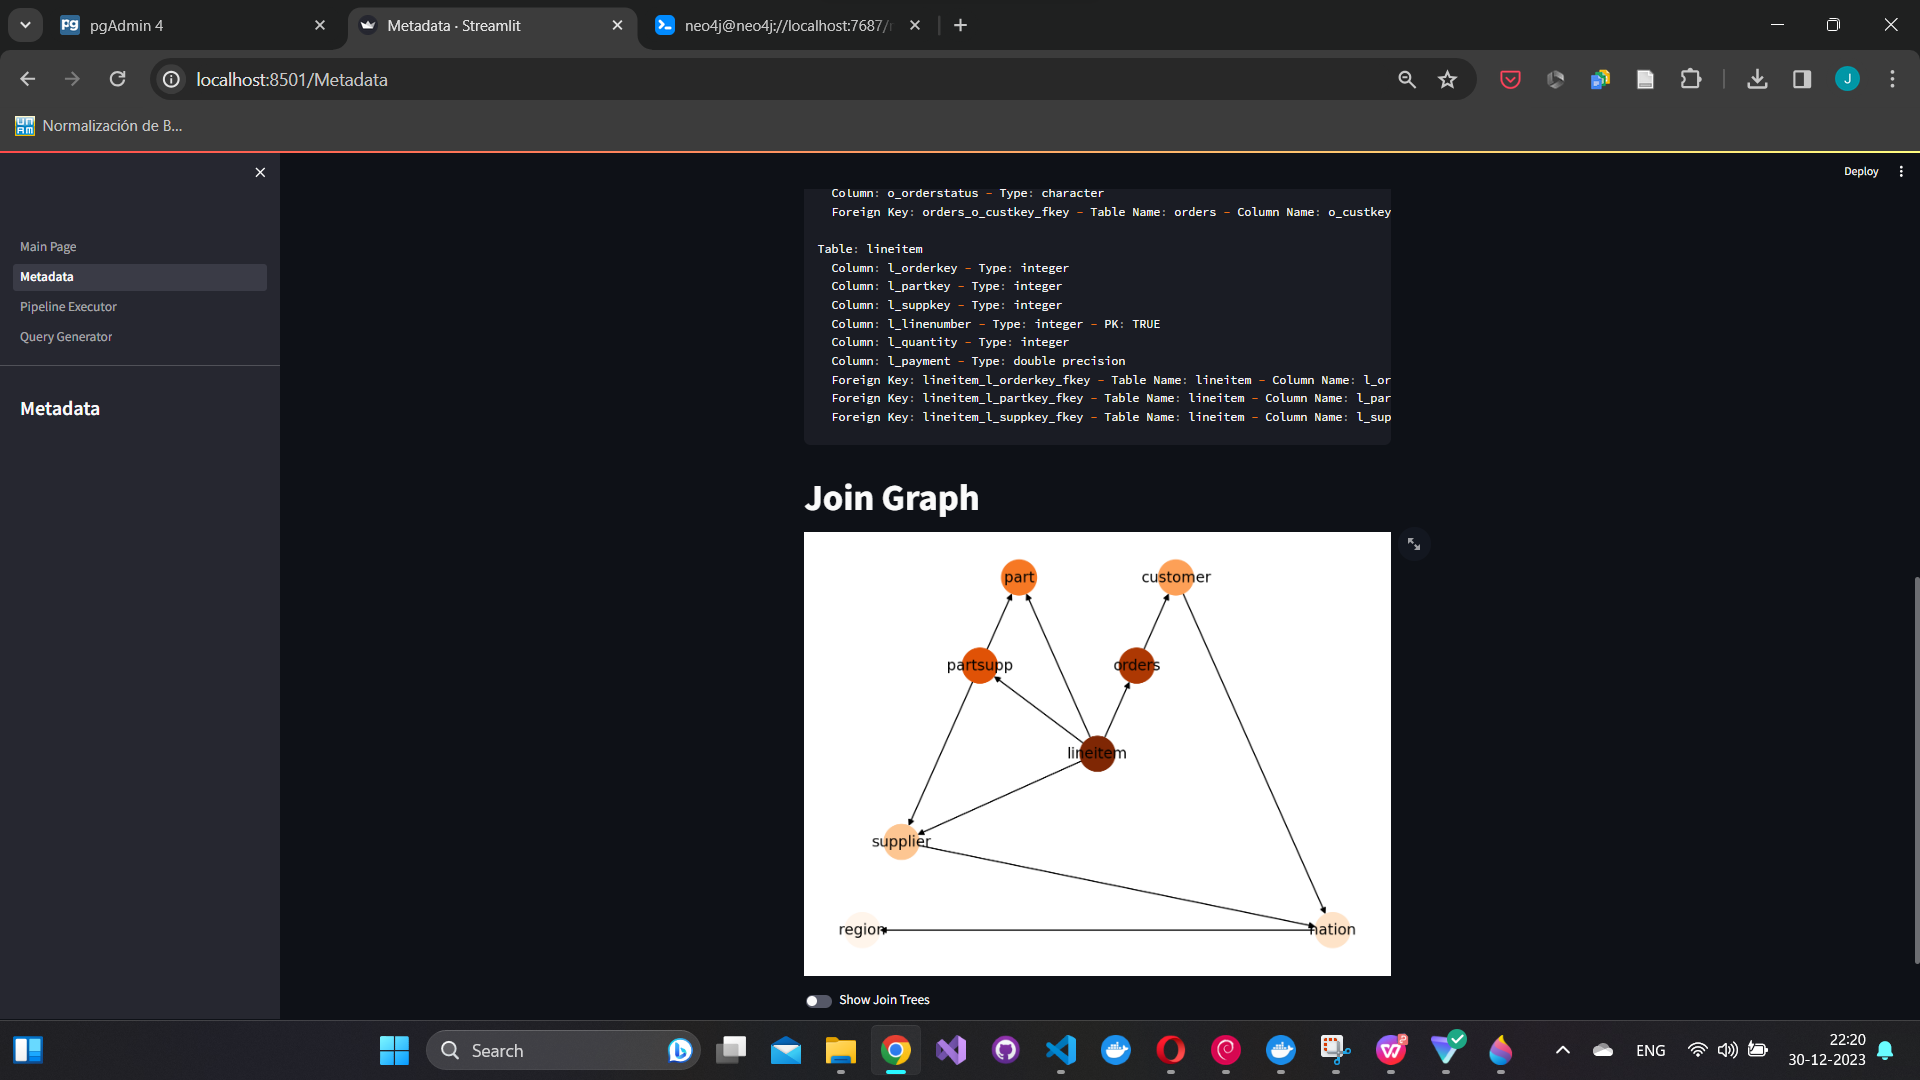
\includegraphics[scale=0.4]{Graphics/metadata.png}
        \caption{Im\'agen de la p\'agina Metadata.}
        \label{fig:meta}
    \end{figure}

    \begin{figure}
        \centering
        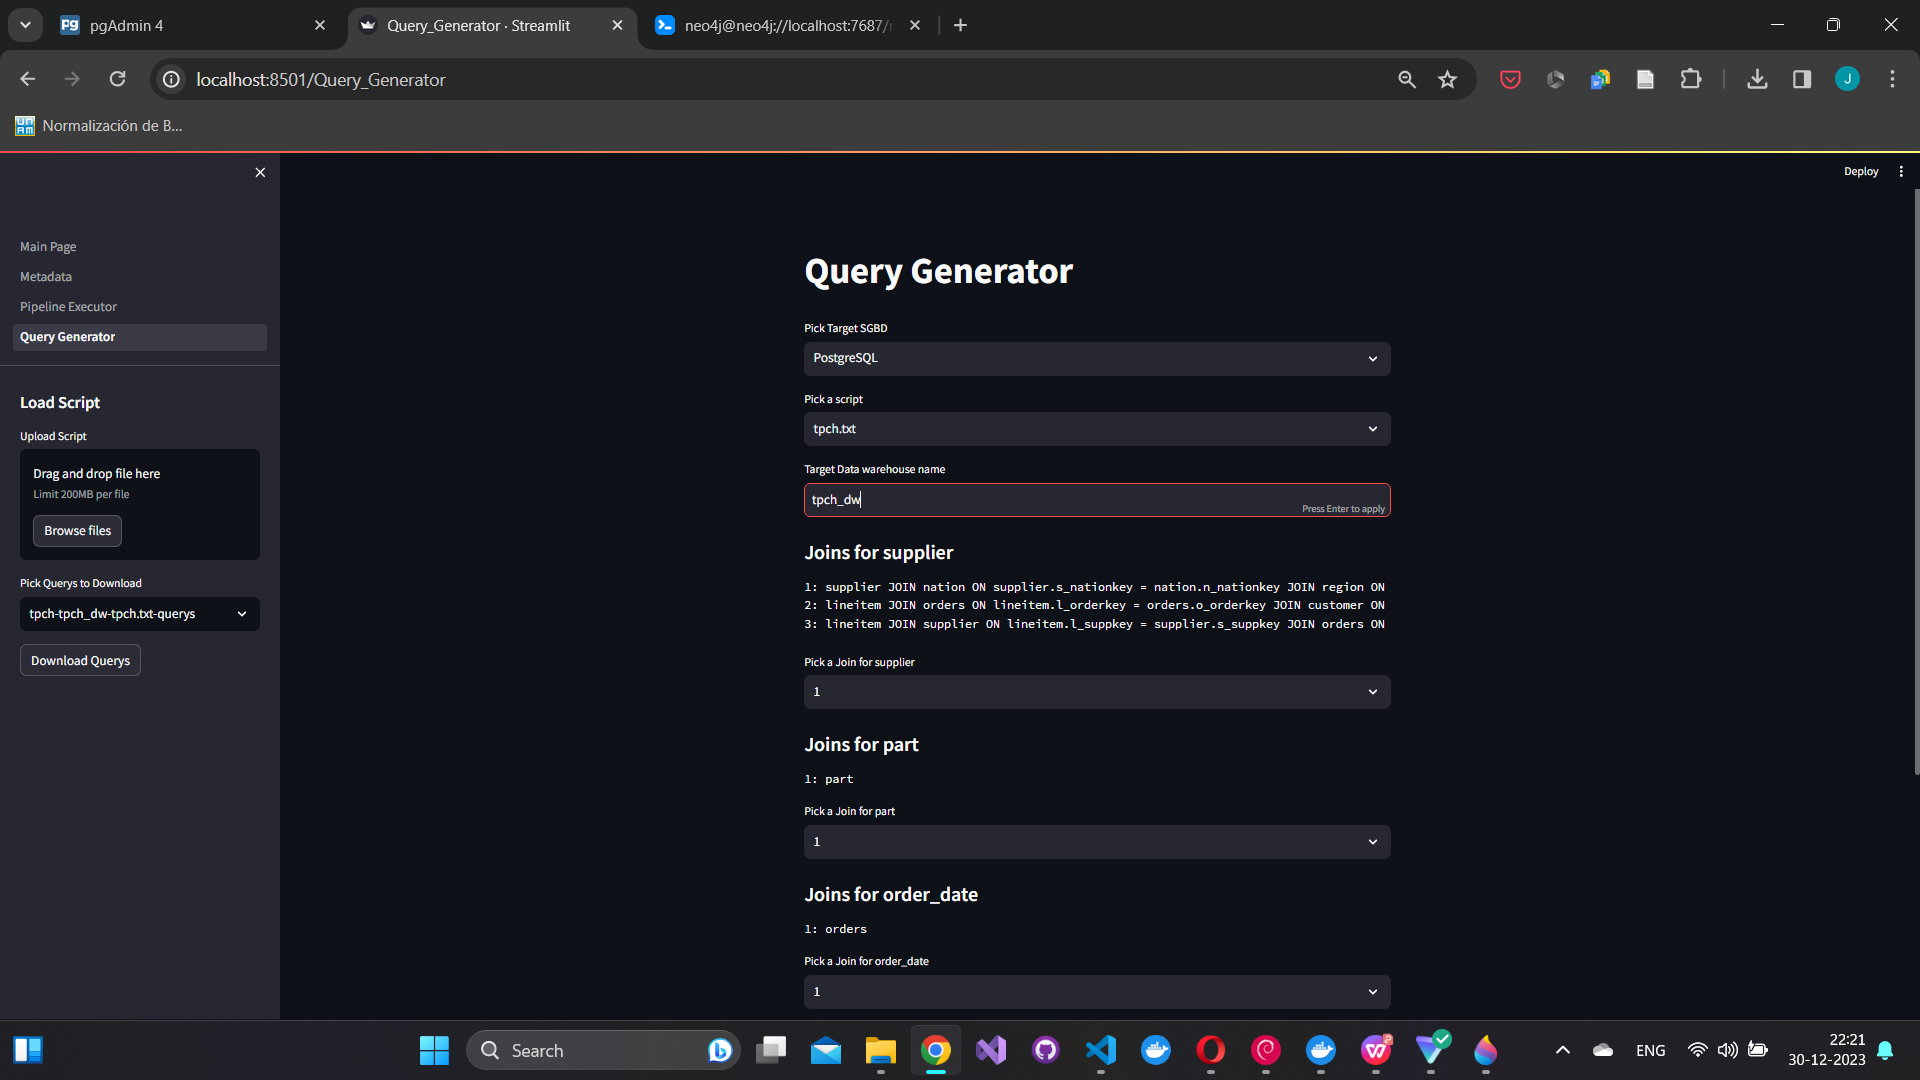
\includegraphics[scale=0.4]{Graphics/querygene.png}
        \caption{Im\'agen de la p\'agina Query Generator.}
        \label{fig:generator}
    \end{figure}

    \begin{figure}
        \centering
        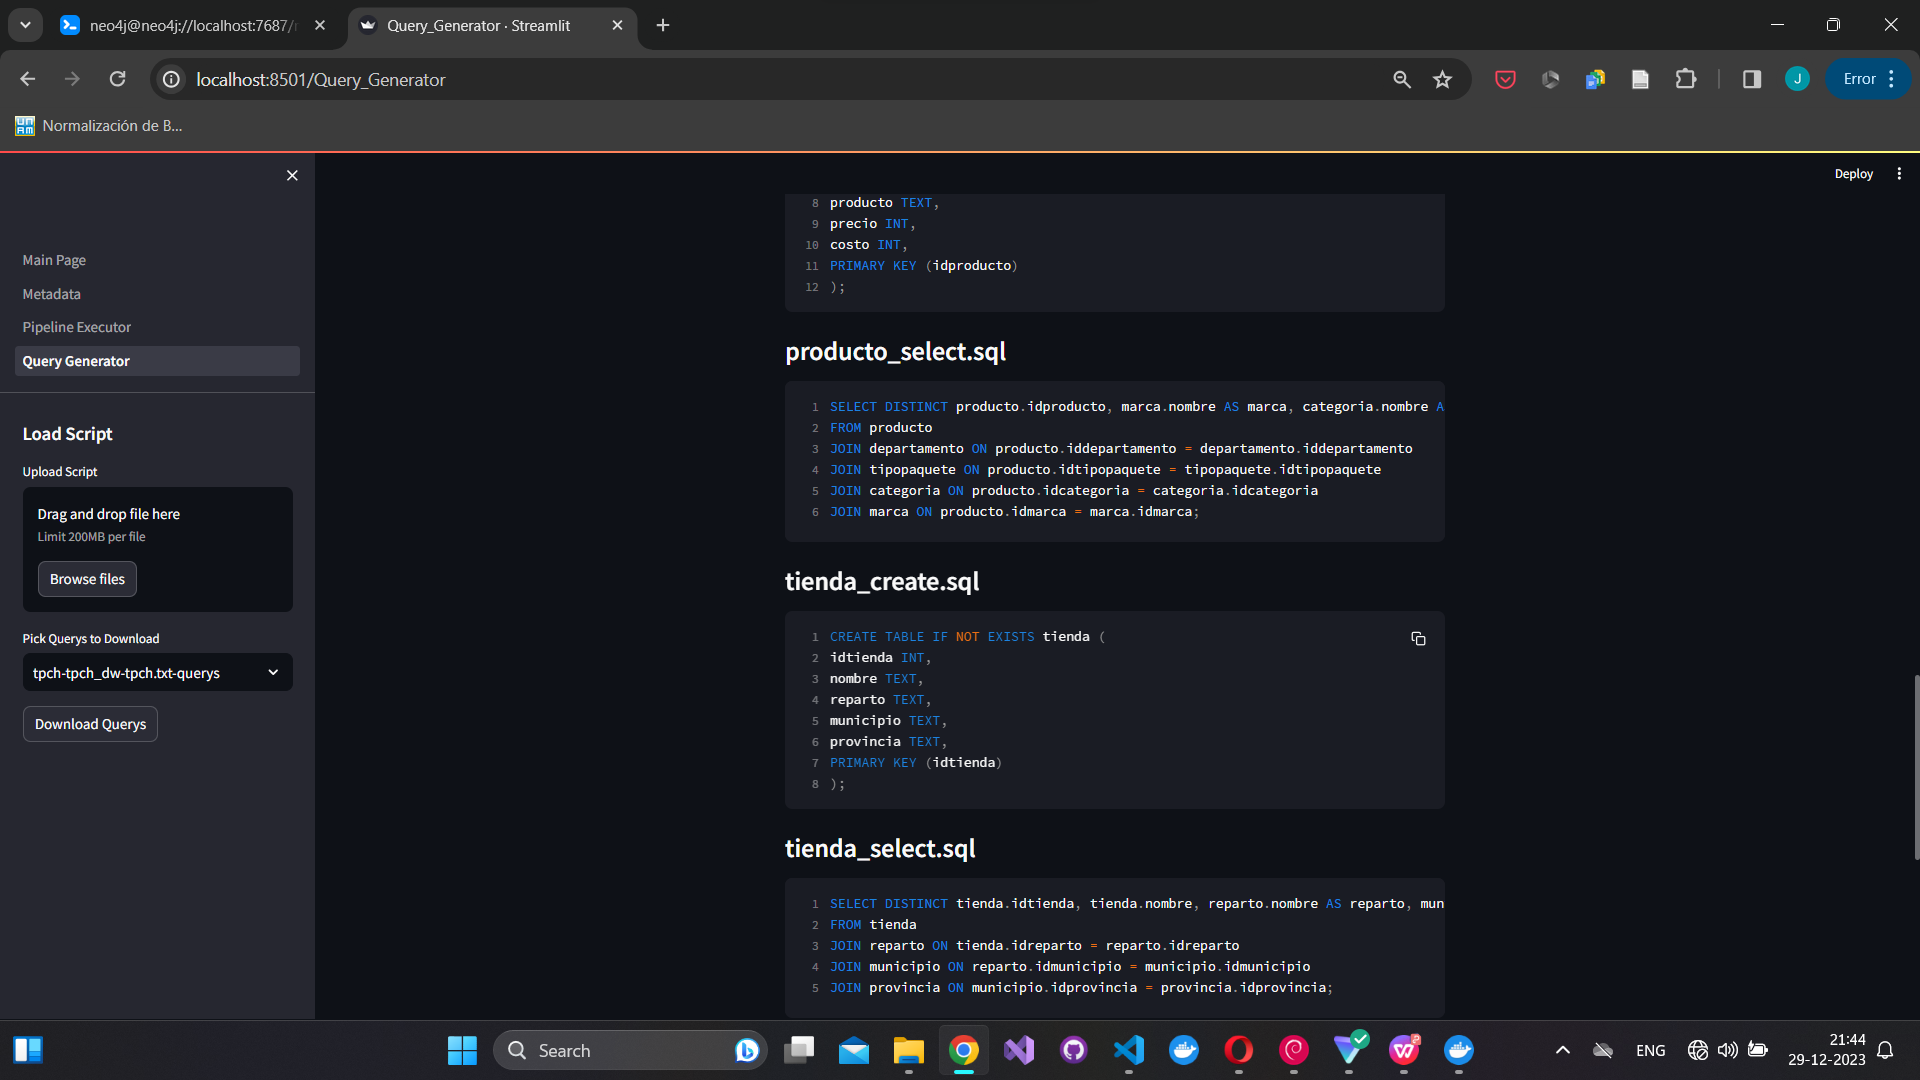
\includegraphics[scale=0.4]{Graphics/generatedquerys1.png}
        \caption{Fragmentos de consultas generadas.}
        \label{fig:qfragment}
    \end{figure}

    \begin{figure}
        \centering
        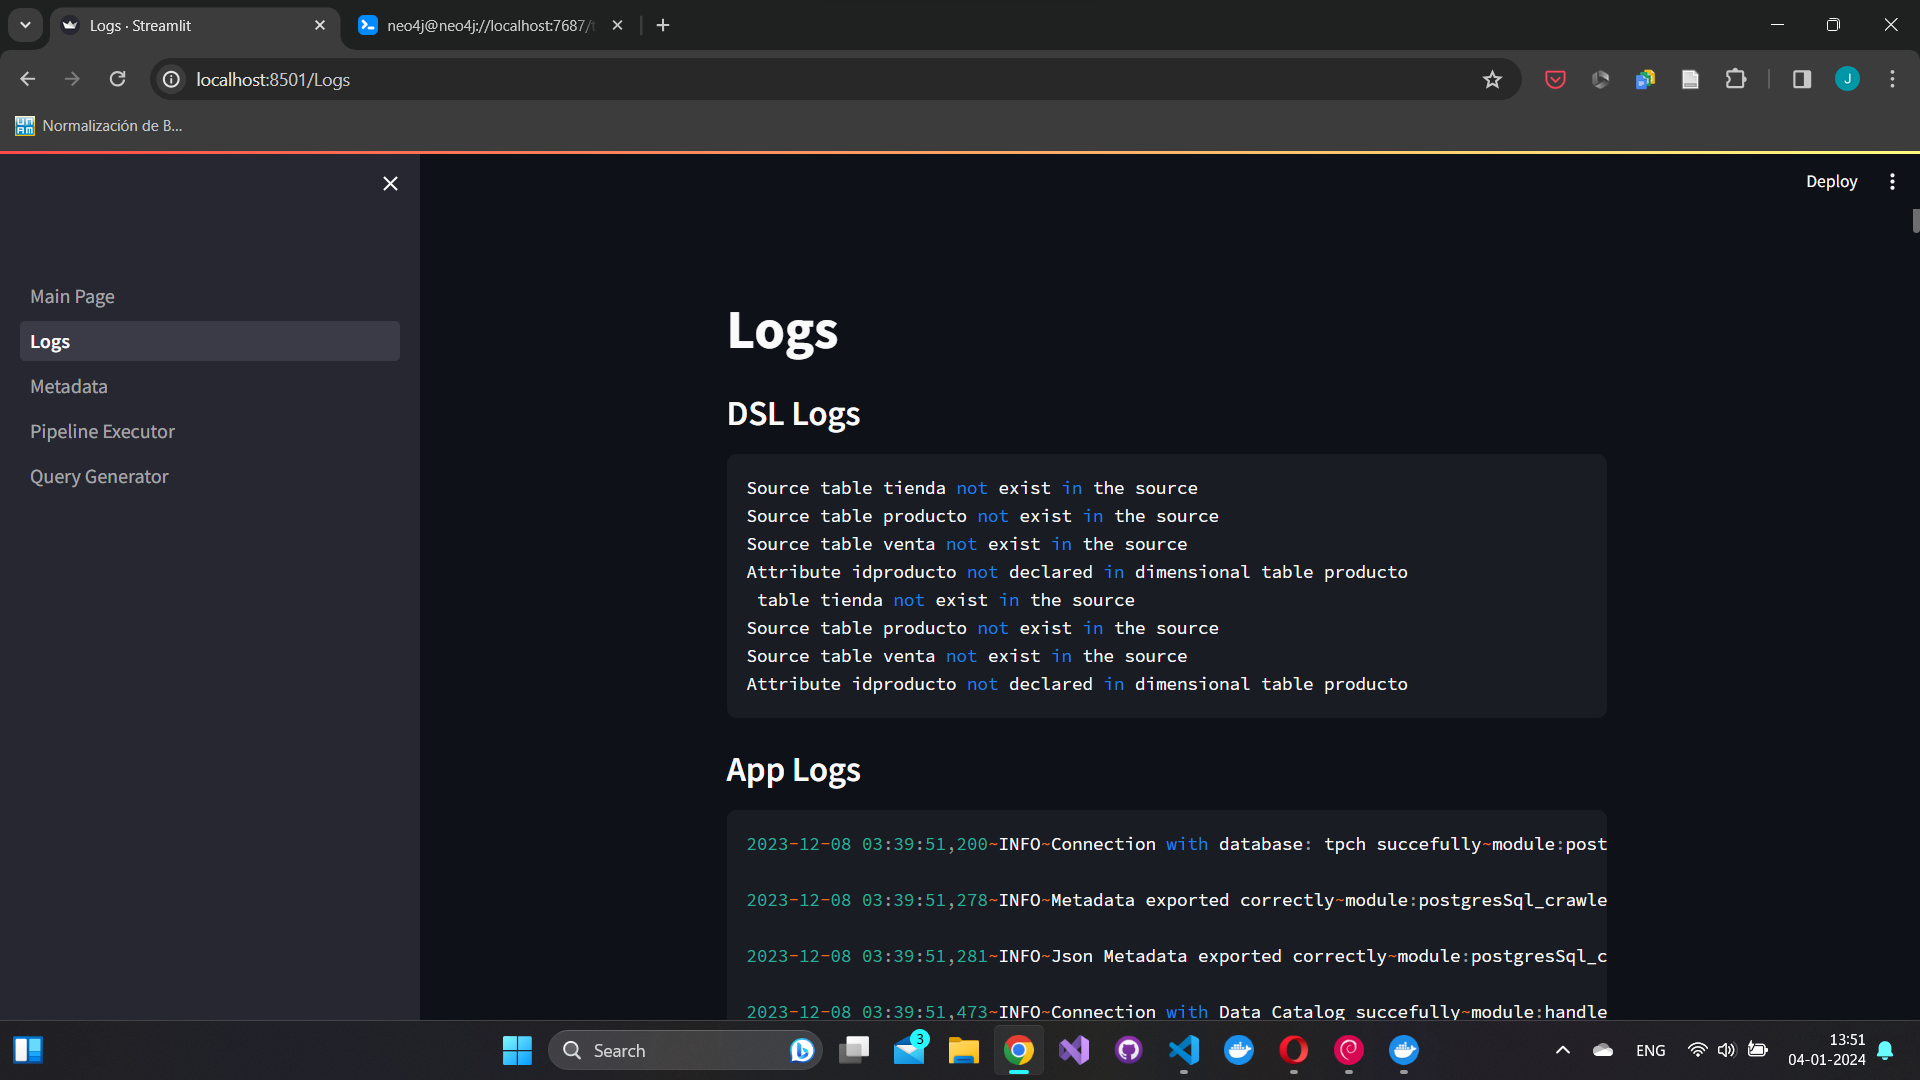
\includegraphics[scale=0.4]{Graphics/logs.png}
        \caption{Im\'agen de la p\'agina Logs.}
        \label{fig:logs}
    \end{figure}
\end{annexes}
%%\printbibliography[heading=bibintoc]

\nocite{*}
\bibliographystyle{plain} % We choose the "plain" reference style
    

\end{document}